\documentclass[border=3mm]{standalone}
\usepackage{tikz}
\usetikzlibrary{cd}
\usetikzlibrary{calc}
\usetikzlibrary{arrows}
\begin{document}

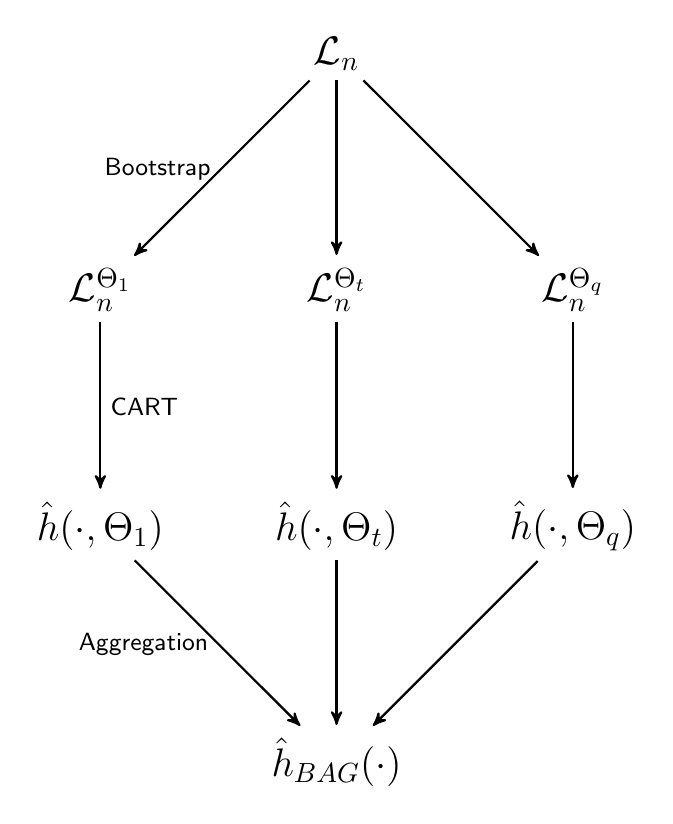
\begin{tikzpicture}[->,>=stealth',shorten >=1pt,auto,node distance=3cm,
thick,main node/.style={font=\sffamily\Large\bfseries}]

\node[main node] (Ln) {${\cal L}_n$};
\node[main node] (Ltt) [below  of=Ln] {${\cal L}^{\Theta_t}_n$};
\node[main node] (Lt1) [left of=Ltt] {${\cal L}^{\Theta_1}_n$};
\node[main node] (Ltq) [right of=Ltt] {${\cal L}^{\Theta_q}_n$};
\node[main node] (h1) [below of=Lt1] {$\hat{h}(\cdot,\Theta_1)$};
\node[main node] (ht) [below of=Ltt] {$\hat{h}(\cdot,\Theta_t)$};
\node[main node] (hq) [below of=Ltq] {$\hat{h}(\cdot,\Theta_q)$};
\node[main node] (hb) [below of=ht] {$\hat{h}_{BAG}(\cdot)$};

\path[every node/.style={font=\sffamily\small}]
(Ln) edge node [left] {Bootstrap} (Lt1)
(Ln) edge node  {} (Ltt)
(Ln) edge node {} (Ltq)
(Lt1) edge node {CART} (h1)
(Ltt) edge node {}  (ht)
(Ltq) edge node {} (hq)
(h1) edge node [left] {Aggregation} (hb)
(ht) edge node {} (hb)
(hq) edge node {} (hb)
;
\end{tikzpicture}


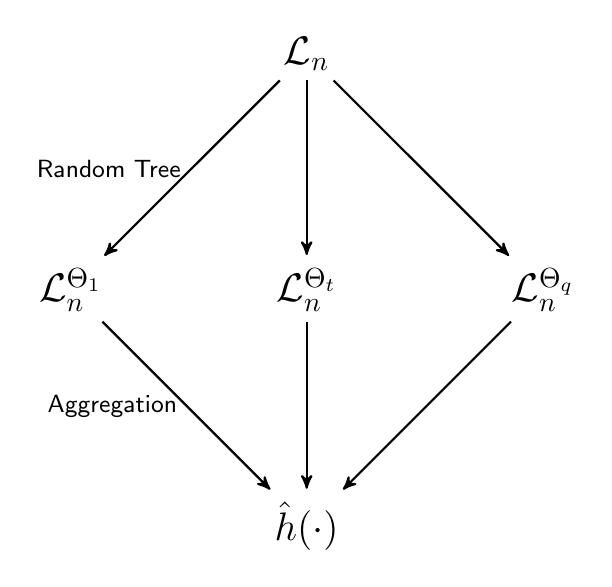
\begin{tikzpicture}[->,>=stealth',shorten >=1pt,auto,node distance=3cm,
	thick,main node/.style={font=\sffamily\Large\bfseries}]
	
	\node[main node] (Ln) {${\cal L}_n$};
	\node[main node] (Ltt) [below  of=Ln] {${\cal L}^{\Theta_t}_n$};
	\node[main node] (Lt1) [left of=Ltt] {${\cal L}^{\Theta_1}_n$};
	\node[main node] (Ltq) [right of=Ltt] {${\cal L}^{\Theta_q}_n$};
	\node[main node] (hb) [below of=Ltt] {$\hat{h}(\cdot)$};
	
	\path[every node/.style={font=\sffamily\small}]
	(Ln) edge node [left] {Random Tree} (Lt1)
	(Ln) edge node  {} (Ltt)
	(Ln) edge node {} (Ltq)
	(Lt1) edge node [left] {Aggregation} (hb)
	(Ltt) edge node {} (hb)
	(Ltq) edge node {} (hb)
	;
\end{tikzpicture}

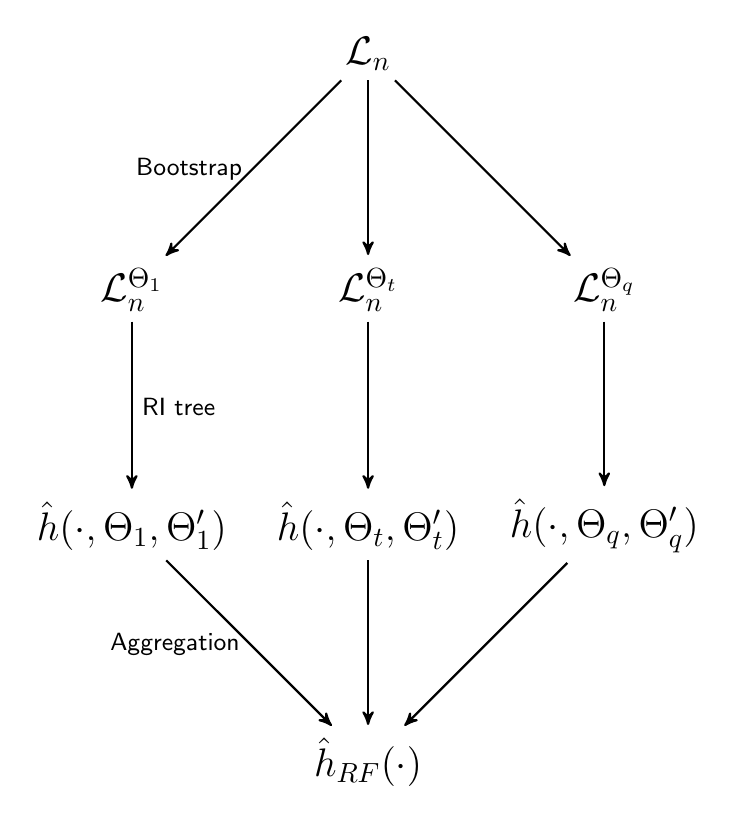
\begin{tikzpicture}[->,>=stealth',shorten >=1pt,auto,node distance=3cm,
	thick,main node/.style={font=\sffamily\Large\bfseries}]
	
	\node[main node] (Ln) {${\cal L}_n$};
	\node[main node] (Ltt) [below  of=Ln] {${\cal L}^{\Theta_t}_n$};
	\node[main node] (Lt1) [left of=Ltt] {${\cal L}^{\Theta_1}_n$};
	\node[main node] (Ltq) [right of=Ltt] {${\cal L}^{\Theta_q}_n$};
	\node[main node] (h1) [below of=Lt1] {$\hat{h}(\cdot,\Theta_1, \Theta'_1)$};
	\node[main node] (ht) [below of=Ltt] {$\hat{h}(\cdot,\Theta_t,\Theta'_t)$};
	\node[main node] (hq) [below of=Ltq] {$\hat{h}(\cdot,\Theta_q,\Theta'_q)$};
	\node[main node] (hb) [below of=ht] {$\hat{h}_{RF}(\cdot)$};
	
	\path[every node/.style={font=\sffamily\small}]
	(Ln) edge node [left] {Bootstrap} (Lt1)
	(Ln) edge node  {} (Ltt)
	(Ln) edge node {} (Ltq)
	(Lt1) edge node {RI tree} (h1)
	(Ltt) edge node {}  (ht)
	(Ltq) edge node {} (hq)
	(h1) edge node [left] {Aggregation} (hb)
	(ht) edge node {} (hb)
	(hq) edge node {} (hb)
	;
\end{tikzpicture}


\end{document}





